\chapter{XRM: A Conceptual Model for XR}
\label{ch:conceptual-model}

According to the bibliographical research in \autoref{sec:background-conceptual}, most of the models described are referred to VEs, indeed there are few works dedicated to the design of mixed experiences. The conceptual model should guide designers in the creation and design of multi-reality and multi-platform experiences in order to build a communication bridge with the team that has to implement the application. Often these are complex systems combining 3D elements, physical objects, "behavior-rich content" \cite{walczak_structured_2008}, devices of different nature, single or shared experiences, indoor or outdoor etc. that severely challenge the developers, especially if they are always compelled to intervene directly on the code. The XR Conceptual Model Framework stems from the need to provide a tool capable of covering different technologies, including VR and AR. The approach used is centered on the human, the protagonist of different scenarios with the support of devices and platforms dependent on the experienced environment. The aim is to create a means to enable high-level development of XR applications, in order to involve also non-experts in the domain. 
In the light of the previous comparative and illustrative analysis, from the variety of conceptual models and based on the planned features, the ISS Model was chosen to inspire the upcoming model. The model of Gianotti et al.~\cite{dobbie_modeling_2020} provided a dual structure that allows for the systematic design of the static and dynamic parts of an XR experience. Although the environments considered have few points in common, the translation of the concepts was not too cumbersome and forced. The XR Conceptual Model Framework is also divided into two parts: a Structural and a Behavioral sub-model, which are described in the next section. 


\section{Structural Model}
\label{sec:conceptual-structural}

The Structural Model is the first part of the XRM Conceptual Model. It comprises all participants in the experience, whether implicit or explicit. They constitute the static modeling part, where the components are selected according to the requirements of the application. The structure elected to represent them is a hierarchy of elements with a top-down concreteness approach, whose levels of abstraction are qualitatively marked and identified by a legend of different colors as seen in Figure \autoref{fig:Legend}. The building blocks in the hierarchy are linked by an "is a" relation, which indicates that between two units one of the two is a generalization of the other. In this way the latter is like a  subclass, a child node that inherits from the father \cite{brachman_what_1983}. This implies that the properties owned by a child node will include its own properties in addition to those owned by the father node which are inherited by the child node. Moreover, there is a 'mereology' relation, or so-called composition relation, which is graphically represented with the shape of a full diamond that indicates how a block combined with others can contribute to compose new ones. 

\begin{figure}[h]
	\centering
	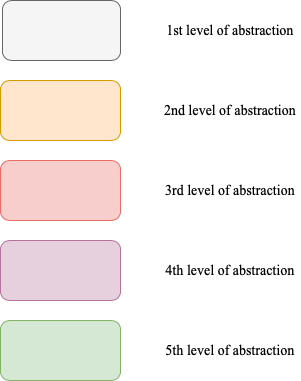
\includegraphics[width=0.5\linewidth]{Figures/Conceptual Model/Legend.png}
	\caption{Legend of levels of abstraction}
	\label{fig:Legend}
\end{figure}

At the summit of the structure stands the entity \emph{Actor}. It embodies a fundamental concept in the field of human-computer interaction, where it is usually considered as a human. In literature it has been defined "as a placeholder for an object when specifying behavior" \cite{de_troyer_conceptual_2007}, i.e. it becomes a way to qualify an abstract object as a system capable of performing actions, stimulating, interacting or reacting to user behavior. The structural model of the XRM Conceptual Model distinguishes in the second abstraction level two macro-categories of Actors as shown in \autoref{fig:ActorHumanNonHuman}.

\begin{figure}[h]
	\centering
	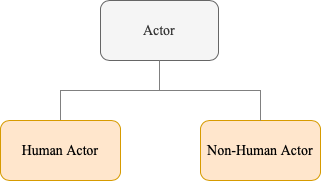
\includegraphics[width=7.5cm]{Figures/Conceptual Model/Actor_Human_NonHuman.png}
	\caption{Structural Model: first two levels of the hierarchy}
	\label{fig:ActorHumanNonHuman}
\end{figure}

\subsection*{Human Actor}
The Human Actor is a type of actor that is generally considered only as a component of the system whose characteristics are crucial in the design process of the interaction with the machine \cite{bannon_discovering_1989}. The presence of a distinction of the Actor between Human and Non-Human arises from the need to elevate the Human from a passive element to an element able to act in an environment, embody and manage a behaviour, rather than being a mere producer of an output information flow. In an interactive system, the Human Actor is nonetheless than the user, the one who uses an application, a device or any technological system through which they perform actions. 

\subsection*{Non-Human Actor}
The Non-Human Actor collects different types of actors, each one with characteristics that must be specified at the design stage. With this term we want to include all the technological components of a system that participate in the interaction allowing the Human Actor to perform certain actions. The results of the interaction are also visible on them.  We can recognize three main sub-categories of Non-Human Actors (\autoref{fig:NonHumanActors}) together with their properties: Physical Component, Environment and Virtual Object.

\begin{figure}[H]
	\centering
	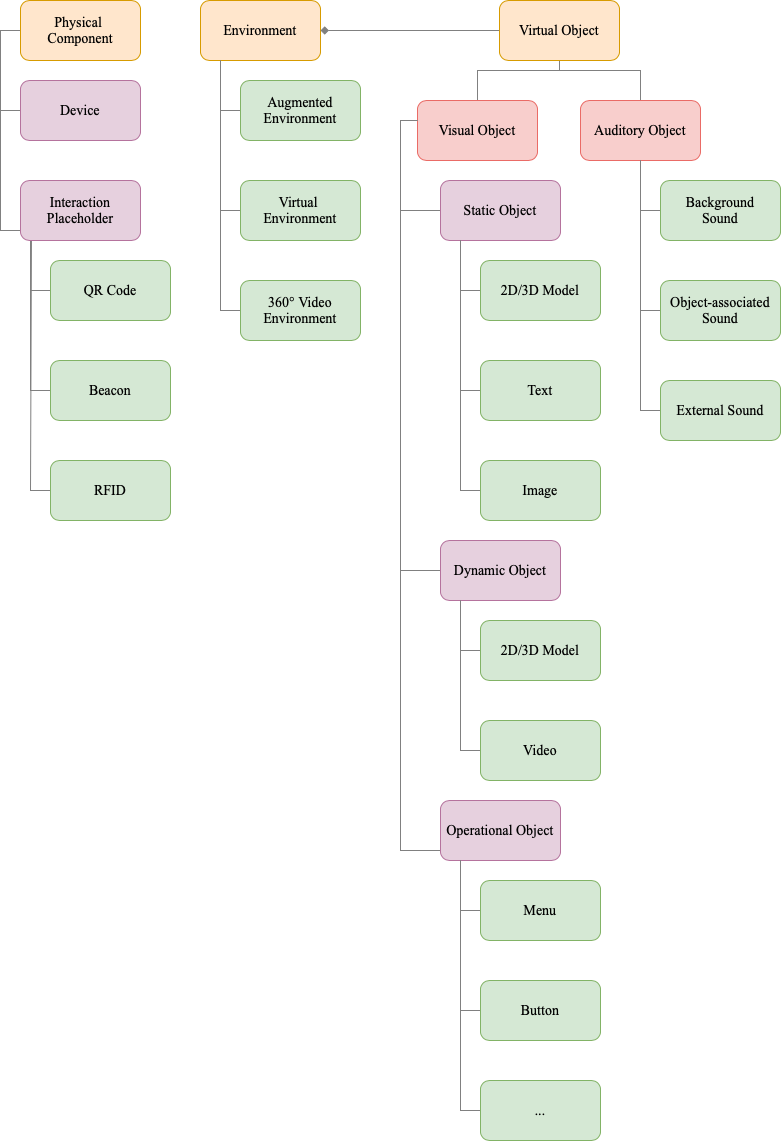
\includegraphics[width=14cm]{Figures/Conceptual Model/NonHumanActors.png}
	\caption{Structural Model - Non-Human Actors hierarchy}
	\label{fig:NonHumanActors}
\end{figure}

\begin{itemize}
    \item \textbf{Physical Component}. Physical Components represent interactive elements with an entirely physical nature, therefore belonging to the real world. They can generate system events or participate in user interactions, receive user commands, trigger other events, etc. \\
    \begin{table}[H]
    \centering
    \begin{tabular}{|l|l|}
    \hline
    \multicolumn{2}{|l|}{\textbf{Physical Component Properties}}                                                                                                \\ \hline
    Id       & It is a unique identification code.                                                                                                              \\ \hline
    Position & \begin{tabular}[c]{@{}l@{}}It is identified by spatial coordinates $(x, y, z)$\\ that locate and track the position of the component.\end{tabular} \\ \hline
    \end{tabular}
    \caption{Structural Model - Physical Component Properties}
    \label{tab:PHCproperties}
    \end{table}
        
    There are two types of Physical Components that we have found:
    \begin{itemize}
        \item \textbf{Interaction Placeholder}. Interaction Placeholders include all identifiable elements i.e. images, codes, symbols such as the QR Code that are recognized by the camera of the device in order to trigger an effect on another Non-Human Actor. However, other devices such as Beacons and RFIDs are also included in this category.
        \item \textbf{Device}: Devices are represented by all the Physical Components that can run an application in XR, whether it is VR or AR. They can be of different nature depending on the technology involved in the designed experience. One or more devices can be included depending on the interaction to be performed. Examples include smartphones, tablets, viewers, card-boards, HMDs, etc.
    \end{itemize}
    \item \textbf{Environment}: Environment represents an element that can have a dual nature. It can identify the real world that can be made of physical objects combined with virtual ones. Otherwise, it can be represented by a world seen through a networked application, a tool supported by a device chosen according to the type of experience designed for the user. In the latter case, the Environment is characterized by a fundamental element: the camera, a device that captures and shows the world to the player. Often the Environment, independently from its nature, is identified with the term "scene", in other cases, instead, the word scene is used to identify the different sub-parts in which it is divided. In this model we will always use only the term 'Environment' in order to avoid any ambiguity. \\
    \begin{table}[H]
    \centering
    \begin{tabular}{|l|l|}
    \hline
    \multicolumn{2}{|l|}{\textbf{Environment Properties}} \\ \hline
    \begin{tabular}[c]{@{}l@{}}Camera \\ Position\end{tabular} &
      \begin{tabular}[c]{@{}l@{}}It is identified by spatial coordinates ($x, y, z$) \\ that locate and track the position of the camera.\end{tabular} \\ \hline
    \begin{tabular}[c]{@{}l@{}}Camera \\ Orientation\end{tabular} &
      \begin{tabular}[c]{@{}l@{}}It is identified by polar coordinates ($\rho$, $\phi$, $\gamma$) \\ that locate and track the camera orientation.\end{tabular} \\ \hline
    Visibility &
      \begin{tabular}[c]{@{}l@{}}It enables or disables the possibility for the user \\ to see the Environment. When in Off mode, the \\ Environment has been triggered but is not visible, \\ i.e. it is hidden from the user's view.\end{tabular} \\ \hline
    \end{tabular}
    \caption{Structural Model - Environment properties}
    \label{tab:Envproperties}
    \end{table}

    The Environment element has three sub-categories:
    \begin{itemize}
        \item \textbf{Augmented Environment}. Augmented Environment (AE) places virtual components in a physical environment. Anchors are virtual elements that the software associates with real elements and that it can recognise, and thus build the experience around the real world by integrating it with the virtual one. Furthermore, AE encapsulates the concept of physical (external) space dimensions, represented as coordinates. It also adds three dimensions where otherwise there would only be one layer superimposed on the users' camera.\\
        \begin{table}[H]
        \centering
        \begin{tabular}{|l|l|}
        \hline
        \multicolumn{2}{|l|}{\textbf{Augmented Environment Properties}}                                                     \\ \hline
        World Anchors & \begin{tabular}[c]{@{}l@{}}They are used by the AR experience\\ to locate the content.\end{tabular} \\ \hline
        \end{tabular}
        \caption{Augmented Environment Properties}
        \label{tab:AEproperties}
        \end{table}
        
        \item \textbf{Virtual Environment}. Virtual Environment  is a completely digital environment that has the characteristic to be navigated and interacted with by the users, of which one or more of their five senses are simulated in real-time \cite{guttentag_virtual_2020}. It places the virtual objects  according to a pure virtual concept of dimensions.
        \begin{table}[H]
        \centering
        \begin{tabular}{|l|l|}
        \hline
        \multicolumn{2}{|l|}{\textbf{Virtual Environment Properties}}                                                       \\ \hline
        World Anchors & \begin{tabular}[c]{@{}l@{}}They are used by the VR experience\\ to locate the content.\end{tabular} \\ \hline
        \end{tabular}
        \caption{Virtual Environment Properties}
        \label{tab:VEproperties}
        \end{table}
        \item \textbf{360$^{\circ}$ Video Environment}. 360$^{\circ}$ Video Environment is represented by a VE that can only be navigated by rotating the device and interacted by buttons superimposed onto the video. The position of the user cannot be changed and overlaps with the position of the camera.\\
        \begin{table}[h]
        \centering
        \begin{tabular}{|l|l|}
        \hline
        \multicolumn{2}{|l|}{\textbf{360$^{\circ}$ Video Environment Properties}}                                           \\ \hline
        Duration & \begin{tabular}[c]{@{}l@{}}It indicates the amount of time\\ the 360$^{\circ}$ Video takes.\end{tabular} \\ \hline
        \end{tabular}
        \caption{360$^{\circ}$ Video Environment Properties}
        \label{tab:360VEproperties}
        \end{table}
    \end{itemize}
    \item \textbf{Virtual Object}. Virtual Object compose the Environment and represent computer-generated elements that simulate real elements and with which the user can interact. Virtual Object in the hierarchy shown (\autoref{fig:NonHumanActors}) is linked to Environment by a "part of" relationship which, as mentioned above, is meant to emphasize that an entity is composed of sub-entities.\\
    \begin{table}[ht]
    \centering
    \begin{tabular}{|l|l|}
    \hline
    \multicolumn{2}{|l|}{\textbf{Virtual Object Properties}}  \\ \hline
    \multirow{4}{*}{Position} &
      \begin{tabular}[c]{@{}l@{}}It is identified by spatial coordinates that \\ locate and track the position of the Virtual Object. \\ These coordinates can be of three types:\end{tabular} \\ \cline{2-2} 
     & Absolute ($x$, $y$, $z$)                               \\ \cline{2-2} 
     & Component-related ($\Delta x$, $\Delta y$, $\Delta z$) \\ \cline{2-2} 
     & User-related ($\Delta x$, $\Delta y$, $\Delta z$)      \\ \hline
    Orientation &
      \begin{tabular}[c]{@{}l@{}}It is identified by polar coordinates ($\rho$, $\phi$, $\gamma$) that \\ locate and track the orientation of the Virtual Object.\end{tabular} \\ \hline
    \end{tabular}
    \caption{Virtual Object Properties}
    \label{tab:VOproperties}
    \end{table}
    Virtual Objects have an additional level of abstraction that characterizes them qualitatively, that is, according to their visual or auditory qualities:
   
   \textbf{Visual Object}. Visual Object encloses a set of Virtual Objects that react to interaction with the user by mainly changing their external characteristics.
    \begin{longtable}[c]{|l|l|l|}
    \hline
    \multicolumn{3}{|l|}{\textbf{Visual Object Properties}} \\ \hline
    \endhead
    %
    \multicolumn{2}{|l|}{Geometry} &
      \begin{tabular}[c]{@{}l@{}}It refers to the representation of the surface, \\ based on mathematical coordinates, that an object \\ can assume. Depending on whether it takes on two or three \\ dimensions, it is called 2D or 3D geometry respectively.\end{tabular} \\ \hline
    \multicolumn{2}{|l|}{Visibility} &
      \begin{tabular}[c]{@{}l@{}}It enables or disables the possibility for the user to see a \\ Visual Object. When in Off mode, the Visual Object has \\ been triggered but is not visible, i.e. it is hidden from \\ the user's view.\end{tabular} \\ \hline
    \multicolumn{2}{|l|}{Scale Factor} &
      \begin{tabular}[c]{@{}l@{}}spatial coordinates (x, y, z) that allow to reduce or increase \\ the size of a Visual Object.\end{tabular} \\ \hline
    \multicolumn{2}{|l|}{Opacity} &
      \begin{tabular}[c]{@{}l@{}}It increases or decreases in percentage the possibility for \\ the user to see a Visual Object. When set to 100\%, the \\ Visual Object has been triggered but is not visible, \\ i.e. it is hidden from the user's view.\end{tabular} \\ \hline
    \multicolumn{2}{|l|}{Selectable} &
      \begin{tabular}[c]{@{}l@{}}It enables or disables the possibility for the user to interact \\ with a Visual Object if the design requires that the object be \\ selected before an action can be performed. When in Off mode, \\ the Visual Object is visible but not interactive, \\ i.e. it does not respond to user commands.\end{tabular} \\ \hline
    \multicolumn{2}{|l|}{Blinking} &
      \begin{tabular}[c]{@{}l@{}}It enables or disables the possibility for the user to see a \\ Visual Object surrounded by a luminous border. When in \\ Off mode, the Visual Object is visible but the luminous border \\ is hidden from the user. This is used, for example, to draw the \\ user's attention to a certain object.\end{tabular} \\ \hline
     &
      Frequency &
      \begin{tabular}[c]{@{}l@{}}It determines the number of times the Visual Object blinks \\ per unit of time.\end{tabular} \\ \hline
     &
      Colour &
      \begin{tabular}[c]{@{}l@{}}It represents the chromatic shade that the light around the \\ Visual Object takes on.\end{tabular} \\ \hline
    \caption{Visual Object Properties}
    \label{tab:VIOtable}\\
    \end{longtable}
    Visual Objects are divided into three subsets: 
    \begin{itemize}
        \item \textbf{Static Object}. Static Object is a Visual Object that is not characterised by movement or animation. We distinguish three types of Static Objects:
        \begin{itemize}
            \item \textbf{2D/3D Model}: 2D/3D Model is a mathematical representation of a two- or three-dimensional object, i.e. a 2D/3D computer-generated geometry.
            \begin{table}[h]
            \centering
            \begin{tabular}{|l|l|}
            \hline
            \multicolumn{2}{|l|}{\textbf{2D/3D Model Properties}} \\ \hline
            Texture &
              \begin{tabular}[c]{@{}l@{}}It is a two-dimensional image in raster format that is \\ reproduced on one or more faces of a multidimensional model. \\ It corresponds to the chromatic variations \\ that a Model may present on the surface.\end{tabular} \\ \hline
            \end{tabular}
            \caption{2D/3D Model Properties}
            \label{tab:2d3dMproperties}
            \end{table}
            \item \textbf{Image}: Image is a visual representation enclosed in a two-dimensional window
            \item \textbf{Text}: Text is a visual description enclosed in a two-dimensional window.\\
            \begin{table}[H]
            \centering
            \begin{tabular}{|l|l|}
            \hline
            \multicolumn{2}{|l|}{\textbf{Text Properties}} \\ \hline
            Offset &
              \begin{tabular}[c]{@{}l@{}}it increases or decreases the user's ability \\ to see Text. When Offset is not set to 100\%, \\ the Text has been triggered but is not visible in full, \\ i.e. a portion is hidden from the user's view.\end{tabular} \\ \hline
            Language &
              \begin{tabular}[c]{@{}l@{}}It allows the user to switch the translation of the \\ Text based on user preferences.\end{tabular} \\ \hline
            \end{tabular}
            \caption{Text Properties}
            \label{tab:Textproperties}
            \end{table}
        \end{itemize}
        \item \textbf{Dynamic Object}. Dynamic Object is a Visual Object that is characterised by movement or animation.\\
        \begin{table}[H]
        \centering
        \begin{tabular}{|l|l|}
        \hline
        \multicolumn{2}{|l|}{\textbf{Dynamic Properties}}                                                                        \\ \hline
        Loop     & \begin{tabular}[c]{@{}l@{}}It enables the cyclic reproduction of a \\ Dynamic Object.\end{tabular} \\ \hline
        Duration & \begin{tabular}[c]{@{}l@{}}It keeps updates the amount of play time of a \\ Dynamic Object.\end{tabular}        \\ \hline
        \end{tabular}
        \caption{Dynamic Properties}
        \label{tab:Dynproperties}
        \end{table}
        There are two types of Dynamic Objects:
        \begin{itemize}
            \item \textbf{2D/3D Model}. 2D/3D Model is a mathematical representation of a two-dimensional/three-dimensional object, i.e. a 2D/3D computer-generated geometry.
            \item \textbf{Video}. Video is a visual reproduction represented in a two-dimensional window.
        \end{itemize}
        \item \textbf{Operational Object}. Operational Object is a Visual Object that allows operations to be carried out and commands to be sent to the system by the user. There are two examples of Operational Objects:
        \begin{itemize}
            \item \textbf{Menu}. Menu consists of a list of elements that can trigger a change of state through a graphical interface, whose geometry can be either 2D or 3D.
            \item \textbf{Button}: Button is a component of the Menu, it allows the user to trigger an event.
        \end{itemize}
    \end{itemize}
    
    \textbf{Auditory Object}. Auditory Object encloses a set of objects that react to interaction with the user with a change in their sound characteristics.\\
	\begin{table}[H]
    \centering
    \begin{tabular}{|l|l|}
    \hline
    \multicolumn{2}{|l|}{\textbf{Auditive Properties}}                                                                                      \\ \hline
    Mute &
      \begin{tabular}[c]{@{}l@{}}It enables or disables the possibility for the user \\ to listen to an Auditory Object. When in Off mode, \\ the Auditory Object has been triggered but cannot \\ be listened to.\end{tabular} \\ \hline
    Duration & \begin{tabular}[c]{@{}l@{}}It allows the user to switch the language of the \\ sound based on user preferences.\end{tabular} \\ \hline
    Loop     & It enables the cyclic playback of an Auditory Object.                                                                        \\ \hline
    \end{tabular}
    \caption{Auditive Properties}
    \label{tab:Audproperties}
    \end{table}
    Auditory Objects are distinguished on the basis of the source from which the sound is reproduced:
    \begin{itemize}
        \item \textbf{Background Sound}: Background Sound is a secondary sound that is activated to complement the experience or part of it, it can be for example a soundtrack etc.
        \item \textbf{Object-associated Sound}: Object-associated Sound is a sound that is linked to the object with which the user is interacting, it can be for example a short sound that provides feedback to indicate the status of the action carried out, such as a timer that signals that time is up.
        \item \textbf{External Sound}: External Sound is a sound from a third party source such as the voice of the tour guide etc.
    \end{itemize}
\end{itemize}

\section{Behavioral Model}
\label{sec:conceptual-behavioral}
\section{Example of use of XRM: The NURE Use Case}
\label{sec:conceptual-nure-example}